\chaptertitle{12}{手把手教你做定投}

\setcounter{figure}{0}\setcounter{table}{0}
在前面的章节，我们已经了解了优化定投的三种思路。这一章，我们就来了解一下如何构建属于自己的定投计划。

\subsection{制订一份完整的定投计划}
{\heiti 一份完整的定投计划包含哪些内容}

一份完整的定投计划，需要我们根据自己的收入和开支，设定合理的每月定投额度，也需要筛选适合投资的品种，设定好买卖区间。最终我们需要把这些因素全部一一落在纸面上，让任何一个拿到这份计划的人，执行后都可以得出相同的效果。如此，这份定投计划才算完成了。

需要强调的是，最终的计划必须落在纸面上！这样才能让自己每次投资的时候严格遵守计划，避免主观情绪的干扰。

{\heiti 四个步骤，帮你搞定一份完整的定投计划}

第一步：梳理自己的现金流，确定每个月可以定投的金额。

指数基金定投一轮大约需要3年的时间。当然，这是一个平均值，并不是说每次都要3年，有时刚开始投资就遇到牛市，时间自然短些，而有时则需要五六年，但是至少我们要做好投资3年以上的心理准备。如果定投的钱在这3年里会用到，那在很大程度上会影响我们的投资。所以，定投的金额要选得合适。如果定高了，可能会影响我们的正常生活，导致后期由于生活所需被迫卖出基金。

每个月拿出多少钱来进行投资，取决于投资者每个月能剩多少钱，毕竟每个人的收入和开支都不相同。

螺丝钉刚开始定投的时候，每个月的工资收入去掉个人的生活开支，还剩下4000元左右。那么，拿出不超过剩余金额的一半用于定投指数基金，也就是2000元，是比较合适的。

为什么是剩余金额的一半而不是全部呢？这是因为定投指数基金的资金可能在几年的时间内不能被拿来使用，所以得留出一部分钱作为备用金，以备不时之需。

现在，读者就可以来具体分析一下自己或者家庭每个月的收入和开支（可以配合记账来进行），并根据未来用钱的规划（如未来3年是否有大额资金的使用计划等），确定自己大致的定投金额。

第二步：挑选出当前具有投资价值的、被低估的指数基金。

具体的挑选方法我们在前几章讲过了，这里不再赘述。大家也可以参考螺丝钉提供的估值表里的指数基金，选择适合自己的。

第三步：选择熟悉的投资渠道，构建一份定投计划。

首先，选择一个自己熟悉的投资渠道，比如银行，或者蚂蚁财富、天天基金、蛋卷基金等网络平台，或者股票账户。定投的实操步骤及演示详见《指数基金投资指南》第5章，或者在微信公众号“定投十年赚十倍”回复“场外基金”或“场内基金”。

其次，确定自己每月定投的时间和频率，比如在发工资之后的第一个交易日进行定投。频率上，按周定投或者按月定投效果相似，选择适合自己的方式就好。

最后，在计划中把遵循的定投策略，包括什么时候定投、什么时候持有、什么时候卖出，都详细地列出来。只有这样，一份完整的计划才能落实在纸面上，帮助我们在以后的执行过程中严格遵守，避免受到主观情绪的干扰。

第四步：在实践过程中，定期检查、优化。

我们制订了一份可以执行的定投计划，但这并不是终点。一份好的计划永远不是一成不变的，需要我们在实践过程中不断地优化和改进。

为了做好计划的优化，在定投的时候我们需要做好定投记录，方便以后进行总结和回顾。定投记录一般包括定投指数基金的日期、指数基金的品种、操作（买或卖）、指数基金的价格、估值等信息。在定投日期一栏，还可以预先把每个月定投的时间写上，这样可以提醒、督促自己按计划来坚持执行。

优化的方法有很多，在前面的章节中也有过介绍，读者可以结合这些投资技巧，不断优化自己的定投计划。比如，我们知道，指数基金越被低估，投资价值就越高，越值得投资。因此我们可以将每个月定投的金额与估值结合起来，做到越低估买入越多，这样可以进一步提升投资收益。

还有一个帮助我们掌握定投知识的好窍门：计划制订好之后，要能把这份计划向别人讲明白，讲解的内容包括什么是指数基金，指数基金有哪些优势，为什么这样制订定投计划，依据是什么等。一套知识体系，只是看完，能掌握10\%的内容，看完又去实践，能掌握50\%的内容，能向别人讲明白，才算是基本掌握了。另外，向别人讲述的过程，也能够帮助我们对自己的定投计划查漏补缺。

这样，一份简单有效的定投计划就制订出来了。按照这个定投计划定投低估值的指数基金，可以保证一个长期不错的收益率。

\subsection{一个真实的定投案例}
以上这样一个定投计划，能获得多少收益、产生什么效果呢？

这里给大家展示一个真实的定投案例，也是我自己的指数基金定投计划：螺丝钉指数基金组合。

“买什么、怎么买、怎么卖”，一直是定投基金时最让人头疼的问题。

我们通过这本书，简单了解了如何在这三个方面优化定投，获得更好的收益，但是具体到投资的时候，还是有很多琐碎的细节。

截至2016年，螺丝钉已经定投了很长时间指数基金，收益也不错。但是很多朋友在定投指数基金的时候，还是会遇到一些问题，例如怎么挑选品种，具体买多少等。

所以螺丝钉做了一个螺丝钉指数基金组合，用产品的方式来演示如何更好地定投指数基金，也方便投资者定投指数基金。

{\heiti 买什么：以宽基指数为主，以行业指数为辅}

这个组合是一个以低估指数基金为主的组合。螺丝钉指数基金组合挑选品种的核心思路如下。

\begin{itemize}
\item 以优秀策略类宽基指数基金为主，主要是红利、基本面、价值、低波动等策略加权指数基金。
\item 以优秀行业指数基金为辅，优秀行业包括消费、医药、中概互联等长期收益居于前列的优秀行业指数基金。
\end{itemize}

投资最重要的是让自己先活下来。宽基指数基金会有波动，但宽基指数包含各行各业，它们的长期表现是稳定的，组合会以策略类宽基指数基金为主，确保在任何情况下，组合不会受到毁灭性打击。

优秀行业指数基金可以作为组合的补充。这些优秀行业本身长期的增长速度、盈利能力都是很不错的。

在挑选品种的时候，要注意有的品种是相互重合的。例如基本面50、300价值，这两个都是大盘类品种，并且金融地产行业比例都比较高，挑选一个就好。再比如上证红利和中证红利，深证基本面60和深证基本面120，也是彼此重合较大，挑选一个就好。

在不重合的前提下，均衡配置优秀的指数基金品种。

{\heiti 怎么买：低估买入+定期不定额}

确定了要投资的品种，之后就是怎么买的问题了。

我们前面介绍过，指数基金在熊市和牛市的涨跌幅差别巨大。最好在熊市市场低迷的阶段，投资处于低估区域的指数基金。换句话说，对上面挑选出来的好品种，最好是在熊市便宜的阶段投资。

再好的品种，也要买得便宜，这也就是我们常说的“又好又便宜”的原则。前提是先确定好品种，再使用估值，而不是反过来。

在熊市定投的阶段，如果遇到市场继续下跌，指数基金的投资价值还会提升。我们可以适当提高定投的金额，也就是使用定期不定额的技巧。这样可以额外提高一部分收益。具体的定期不定额计算公式，本书前面章节也有介绍。

使用这两种方式，就可以保证我们在挑选到好品种的基础上，以更低的风险获得好收益。

{\heiti 怎么卖：长期持有，牛市高估卖出}

现在，到了卖出的环节。

如果投资者短期内需要用钱，可以在指数基金回到正常估值、有一定收益率的情况下止盈，或者直接按照30\%的收益率止盈。这样可以大概率在2～3年就遇到一次止盈机会，方便短期内用钱。不过按照收益率止盈，需要投资者根据自己的情况来判断。

如果投资者长期不用钱，如3～5年或5年以上不用钱，就可以低估买入，耐心持有指数基金。除非出现牛市后期的高估，其他时间不考虑卖出。通常牛市高估，是7～10年遇到一次，例如A股2000年牛市、2007年牛市、2015年牛市。

低估买入，在正常估值时耐心持有，因为我们买入的是长期盈利增长不错的品种，盈利增长也会给我们带来不错的收益。所以在牛市到来之前，我们的组合已经有不错的收益了。可以结合我们前面章节介绍过的止盈策略来卖出。

这就是螺丝钉指数基金组合，定投指数基金的理念和思路综合运用了各种优化定投收益的方法。

在构建这个组合之前，螺丝钉是自己定投单只指数基金，但挑选基金的思路、定投多少钱、最终收益等都不好统计。有了这个组合之后，就可以更方便地运用定投的技巧了。

{\heiti 螺丝钉组合的收益}

我们来具体看一下，螺丝钉组合的收益率情况。

（1）2016年1月1日至2019年5月1日，螺丝钉指数基金组合跑赢上证指数。

上证指数同期下跌13\%，螺丝钉指数基金组合同期上涨32.9\%。这3年多时间里，螺丝钉指数基金组合跑赢上证指数45.9\%，平均每年跑赢上证指数约11\%。

（2）2016年1月1日至2019年5月1日，螺丝钉指数基金组合跑赢沪深300指数和中证500指数。

沪深300指数同期上涨9.74\%，螺丝钉指数基金组合同期上涨32.9\%，跑赢约23\%。

中证500指数同期下跌27\%，螺丝钉指数基金组合同期上涨32.9\%，跑赢约59.9\%。组合每年跑赢的幅度大小不一。具体如图 \ref{fig:12-1} 所示。

\begin{figure}[htbp]
\centering
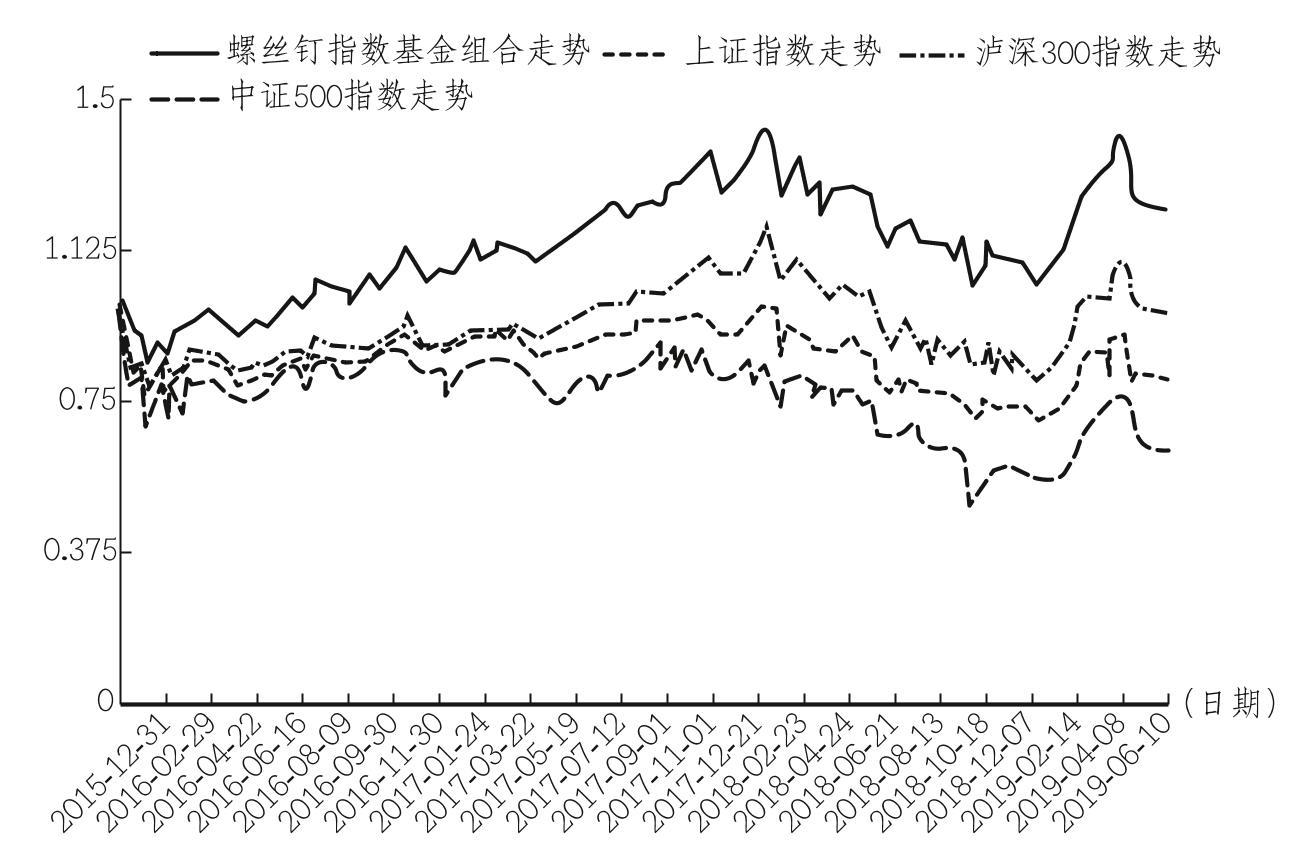
\includegraphics[width=\textwidth,height=0.82\textheight,keepaspectratio]{figure/图12.1.png}
\caption{螺丝钉指数基金组合与上证指数、沪深300指数、中证500指数走势对比}\label{fig:12-1}
\end{figure}

获得更高收益的原因主要是以下两部分。

（1）挑选了长期收益更好的优秀品种。

例如，螺丝钉这几年里投资的优秀策略加权指数基金的收益率高于沪深300指数。

（2）在熊市低估区域投资，越跌越买。

2016—2018年，A股大多数时间里处于下跌，在熊市低估区域投资，符合我们前面说的买价格低于价值品种的理念。并且组合越跌越买，也能获得一些额外的收益。\\

在投资的过程中，也曾经出现在长达半年左右的时间里，组合跑输沪深300、中证500等指数的情况。这也是很常见的。

比如说我们前面介绍过的一些跑赢沪深300指数、中证500指数的策略指数，但通常是一年里，7个月跑赢、5个月跑输。这些策略指数不会每段时间都是跑赢的，但是时间拉长了，其收益率仍然有优势。

随着A股逐渐成熟，螺丝钉指数基金组合未来可能每年跑赢沪深300指数和中证500指数3\%～5\%。

每年3\%～5\%的超额年化收益率，复利积累起来，最后组合是可以大幅战胜沪深300和中证500指数基金的。

从2016年到2019年，A股是一个整体下跌的过程。在这个过程中，我们也可以获得正的收益，等到了像2007年和2015年那样的牛市阶段，收益还会有一个质的飞跃。

这是一个真实的定投指数基金的案例。这个组合也会长期运作下去，为普通投资者定投指数基金，起到一个参考作用。

如果投资者不想思考复杂的指数基金定投计划，可以直接跟投这个螺丝钉指数基金组合。在螺丝钉的微信公众号“定投十年赚十倍”上回复“螺丝钉组合”，可以看到具体跟投方法，以及最新的组合持仓和投资收益介绍。

在定投过程中，投资者可能会面临各种不同的需求。这里用三个实例，讲解一下三种最有代表性的定投需求，以及如何针对不同需求制订相应的定投计划。这三个实例分别是为父母构建养老定投计划，为自己构建加薪定投计划，为孩子构建教育定投计划。这三个计划都以1000元作为初始投资资金。

不管是什么需求，定投过程中“买什么、怎么买、怎么卖”这几点基本不变。读者可以参考这三个实例，更好地完善自己的定投计划。

\subsection{如何帮父母更好地养老}
{\kaishu 我父亲有一笔40万元的养老金，如何帮他做资产配置？全部买货币基金可以吗？}

全部买货币基金会有点儿吃亏，因为货币基金是肯定跑不赢通货膨胀的。

货币基金的优势在于：它基本上不会亏损。

长期不用的钱，其实挺适合配置低估指数基金的。不过父母年纪大了，抗风险能力、对市场波动的接受程度可能都会低很多。

下面介绍几种帮父母养老的办法。

{\heiti 30\%左右的存量资金，配置指数基金}

我们可以用“100-年龄”的方式，来决定配置指数基金的比例。

比如说父亲60多岁，接近70岁了，那就可以直接用30\%的资金，也就是12万左右，来投资低估指数基金。

投资指数基金的这部分资金又可以分成20份，按月分批配置低估的指数基金。

对养老来说，低估的红利类指数基金是很合适的选择。或者直接投资螺丝钉指数基金组合，这个组合就是一篮子低估的指数基金，一键投资也非常方便。不过组合是按周来定投的，那这部分资金可以分为80份来按周分批定投。

剩下的28万元，可以配置银行理财产品、货币基金等品种，力求稳定。

这样，这笔资产的配置情况如下。

\begin{itemize}
\item 指数基金部分，长期来看可以跑赢通货膨胀，用来长期增值。
\item 银行理财产品和货币基金部分，可以用来应付日常生活的支出。
\end{itemize}

不过上面这种做法，前提是父母明白指数基金的投资价值，有能力长期投资。有的时候父母是不敢投股票市场的，他们害怕有风险，把养老的钱损失掉了。这时我们就需要一个更稳妥的投资方法：保本投资组合。

{\heiti 用CPPI策略制订一个“保本投资组合”}

早期余额宝刚出来的时候，曾经流传一个笑话：买1万元的余额宝，用每天的利息买彩票。因为余额宝每天都有利息，用利息买彩票是源源不断的。当然我们掌握了投资的理念后，就知道这只是一个笑话，因为彩票是负收益的，平均投入100元，可能只剩下50元。但是这个原理可以被用在投资上，打造一个保本投资组合。

保本投资策略，比较常见的是CPPI策略，即大部分资金配置货币基金、理财产品、债券，少部分资金配置低估指数基金。

比如说100万元，用90万元配置年收益率为5\%的理财产品，剩下的10万元配置低估指数基金。

一年后，如果股市下跌，低估指数基金跌幅最高为20\%左右，那10万元还剩下8万元，但是理财产品可以获得4.5万元的收益，合计就是90+4.5+8=102.5万元，还是保本的。

如果股市上涨30\%，那10万元会变成13万元，那就是90+4.5+13=107.5万元。

因为指数基金长期上涨，且优秀指数基金的长期年化收益率在10\%以上，比理财、债券等品种的收益还要高，所以这样做大概率收益会更好。同时，兼顾了本金的安全性，所以CPPI策略也被称为保本投资策略。

那这个策略里，指数基金和理财产品的比例怎么确定呢？通常是以稳健的理财产品等品种为主要仓位，以指数基金为小比例的仓位。

比如说低估指数基金，最大跌幅在20\%～30\%，只要理财产品的收益可以覆盖指数基金的最大跌幅，那就不用太担心亏损的问题。

通常来说，配置理财产品的比例为8～9成，剩下的配置低估指数基金，就可以实现类似保本的效果了。遇到市场短期上涨比较多，那最后收益会远高于普通的理财产品的收益。以前市面上的保本基金，基本使用的就是类似的原理。

所以，如果父母不能接受第一种投资方法，用CPPI策略投资也可以。比如说我们不动用40万元的本金，用每年的银行理财产品或者储蓄的利息来投资低估指数基金。这样无论指数基金怎么波动，40万元的本金不会有风险。每年利息投资低估指数基金，时间拉长了收益也不错，至少比单纯存银行好很多。

{\heiti 拿出一部分工资，为父母构建一个养老定投计划}

其实，国内现在养老制度越来越完善，父母退休后都有退休金、养老金，生活并不愁。但父母操劳一辈子，习惯为儿女考虑，不舍得花钱为自己改善生活，提高生活质量。所以我们可以帮他们建立一个养老定投计划，每个月拿出工资的一部分，定期投入一部分钱，用于他们退休后提高生活质量，例如去旅游、买自己想要的东西。

养老定投计划前期不断投入，退休后开始支取。因为退休前有工资收入，而退休后的收入会比退休前有所滑落，所以需要养老定投计划来补充。

养老定投计划可以仿照养老金的方式：退休前一直往计划里定投资金，只进不出；退休后开始有限度地支取，每年提取比例不超过指数基金市值的4\%；每年结余的资金也可以再投入指数基金。

在为养老定投计划选择基金品种时，也应该有一定的倾向性。养老定投计划特别适合构建在高分红的指数基金品种上，例如红利指数基金。因为红利指数基金一般具备高分红的特性，后期依靠指数基金每年的现金分红，就可以稳定获取用作支出的现金，并且指数基金的分红并不受股价涨跌的影响。

所以我们可以为父母养老制订如下定投计划。

（1）确定每月投入养老定投计划中的资金量。

（2）投资低估指数基金或者螺丝钉指数基金组合，或者挑选股息率比较高的指数基金品种。

（3）确定定投日、定投渠道等，再根据个人的需求，决定定投的年限（比如还有多少年退休，大约何时会需要取用资金等）。在此之前进行定投，资金只进不出，达到一定年限后，基金每年的分红收益就可以用来支付生活的相应开支。如果基金没有分红，可以每次卖出不超过4\%的基金份额获得现金，这样不会影响长期取用。

（4）遵循指数基金的投资策略，在指数基金处于低估、值得投资的时候，开始我们的定投计划。

\subsection{如何给子女准备教育金}
{\kaishu 宝宝两岁半，我想给宝宝储备一笔教育基金，该怎么做？一直想定投基金，但是该如何准备呢？}

{\heiti 教育定投的特点}

教育定投有如下几个特点。

（1）需要用钱的时间点非常明确。毕竟子女什么年纪上小学、上大学都能预测到。

（2）从开支的角度，大学开支和留学开支是最大的，所以教育定投主要是为这两项开支做准备。

我们以储备大学教育基金为例，通常子女是18岁上大学，在上述案例中，也就是离用钱还有16年左右。

一轮牛熊市通常是7～10年，如果是离用钱还有16年，那大概率至少会遇到一次牛市。那可以通过定投低估指数基金来积累大学教育基金。下一轮牛市的时候高估卖出，收益会不错的。这段时间内的定投跟普通定投差不多，也可以直接按比例跟投螺丝钉指数基金组合，比较省心。

不过，卖出后再投入的时候，距离用钱可能不到一轮牛熊市了。那就需要放宽卖出的阈值。

比如说之前到高估卖出，现在可能到正常估值就卖出，这样可以两三年就等到投资机会。或者干脆用按收益率止盈的方式，收益率满30\%就卖出。这都是增加卖出的机会，不需要等太长时间，保证资金到用的时候能拿出来。

如果距离使用资金还有2～3年，那就不适合投资低估指数基金了，用银行理财产品等稳妥工具打理就好。

距离用钱的时间越远，低估指数基金越值得考虑；距离用钱的时间越近，那就要考虑稳妥的工具了。

{\heiti 准备教育金的要点}

如何为子女构建教育定投计划，是当前许多年轻父母非常关注的事情。如今养育孩子的成本越来越高，各地尤其是竞争激烈的北上广等大城市，“拼娃”的现象越来越严重。目前送一个孩子去英国读书，平均每年要准备15万～30万元人民币。在北京，一个普通的小学生一年至少也要花费几万元用于报培训班、辅导班等。对现代人来说，子女教育在家庭开销中所占的比重越来越大。

十几年前，银行就开始宣传“教育储蓄”，意图让家长存银行定期，为自己的孩子积累将来教育所需的开支。很明显，定期储蓄的利率一年只有几个点，2015年降息之后，一年期定期储蓄的利率不到2\%（截至2017年6月30日）。靠银行的定期储蓄为子女教育储备资金，实在不是一个好的选择。

教育金有一个很明显区别于其他计划的特点，那就是需要用钱的时间点具有很强的可预见性，且往往在这个可预见的时间点是一次性支出的。所以，准备教育金定投计划时，首先要保证资金在需要使用的时候，一定是以现金的形式存在的，是可以拿来用的，其次才是提高收益。

因此，子女教育金定投计划在卖出条件的设置上要放宽，这样就能等到更多的卖出机会。卖出之后，可以将之转为保本理财产品来打理。虽然收益会低一些，但卖出机会往往在更短的时间里就能等到一次，不会影响资金的提取。

所以，我们可以以此构建如下子女教育金定投计划。

（1）确定教育金定投计划的每月定投金额。

（2）投资低估指数基金或者螺丝钉指数基金组合。

（3）确定定投日、定投渠道等，再根据孩子上学需要用钱的时间，确定定投的年限。

（4）遵循低估买入的策略来定投。如果短期要用钱，可以根据“30\%收益率止盈”，或者进入正常估值后止盈。

{\heiti 如何培养孩子的财商}

对孩子进行财商教育，是现代教育非常缺少的一部分，但实际上这对家庭财富的影响是最大的。有些孩子甚至到了大学毕业，才开始有理财的意识。螺丝钉就是如此，上班之后才开始重视投资理财，但起步还是晚了一些。

小孩子没有收入，也没有生活的压力，暂时不太需要了解具体的投资理财技巧，更重要的拥有正确的理念。

第一个理念，是有正确的消费观，能存下钱。

投资的第一步是存钱。但其实这一步很多人做不到。现在消费信贷产品层出不穷，很多年轻人都是借钱消费。

消费是拿当前的资金，获得即时的满足感。投资是把当前的钱先投到资产上，期望以后增值了再消费获得满足感。任何情况下，消费都比投资更容易。因为消费不需要等待，是一种及时享受。但是同样的钱，去做任何一种投资，都需要时间的沉淀，这就需要我们有足够的耐心。

有些人没有耐心，无法等待长期投资，他们会把钱拿去消费，甚至借钱消费。

所以首先要帮助孩子建立正确的消费观，让他们知道父母赚钱不容易，不能轻易挥霍，自己想要得到什么东西，就得先付出。而且有多少钱，花多少钱，“把钱花在刀刃上”。这样孩子将来至少不会变成月光族或者败家子。

第二个理念，是有攒资产的意识。

可以先从货币基金开始。因为货币基金比较直观，每天都有收益，父母可以买入1000元的货币基金，每周给孩子展示一下账户资产量是在不断增加的。

父母也可以把钱兑换成孩子能直观认知的东西，如玩具等。例如1000元现在可以买100个孩子喜欢的玩具，但如果把1000元买成货币基金，过段时间，就可以买103个孩子喜欢的玩具。

不同类型的资产的差别，其实主要是收益和波动风险，但本质上都是产生现金流、不断增值。让孩子从货币基金开始认识到要攒资产。之后可以再逐渐介绍各种不同资产，收益高的资产有哪些。

上面两个理念，孩子在小学阶段都可以掌握。

第三个理念，是把投资理财的技能，跟自己的人生规划结合起来。

社会财富是逐渐增多的，所以手里的现金会贬值，越来越不值钱。

有些资产可以跑赢通货膨胀，但有些资产是跑不赢通货膨胀的。像货币基金等，虽然很稳健，每天都有收益，但是长期来看是跑不赢通货膨胀的。能跑赢通货膨胀的资产，主要是优质的股票资产、房地产资产、人力资产。

优秀的股票资产，可以从低估指数基金中选择。可以指导孩子用压岁钱做一个按年的定投计划，10年下来，这个计划的收益是很可观的。

优质的房地产。孩子大学毕业之后在哪个城市工作定居，就在哪里买房。年轻人购买首套房产，可以享受很多福利，比如首付比例比较低，还可以用公积金贷款等。很多地方的公积金贷款利率只有3.25\%，这是国家给的一个福利，可以帮家庭减少很多负担。

优秀的人力资产。国内本科学历学生的平均月工资比大专学历学生高，研究生比本科生高。这也是我们要认真学习、考好学校的原因。

要么持有优秀的资产，要么把自己变成优秀的资产，才能跑赢通货膨胀。

这更多是高中阶段和大学阶段的孩子需要拥有的理念，把投资理财的技能跟自己的人生规划结合起来。

\subsection{如何用定投为自己加薪}
{\kaishu 刚毕业进入国企，完全不懂理财这方面的知识，工资只有4000～5000元，每月定投多少钱合适呢？}

在国企工作，收入稳定，意味着现金流很稳定，但收入的增长速度可能不会太快，特别适合采用定投的投资方法。这一阶段收入相对较少，主要以积累经验为主。等有了经验，未来收入提升了，可以再逐渐提高投资比例。

我们可以以此构建一个加薪定投计划。

第一，可以用每月的收入减去各项开支，然后将剩余资金的一半用来投资指数基金。这是一个比较通用的规则。如果金额比较少，也可以固定每个月节约下一部分来定投。

比如说每个月挣5000元，开支2000元，剩下的3000元，可以拿1500元来定投。其余的1500元，可以报学习班、考证，提升自己的竞争力。因为三四十岁之前，努力提升自己的人力资产，也是很重要的。平时也有一些花销需要应对，如果剩余的钱全部拿来投资，也不太合适。具体比例可以根据个人情况来调整。

第二，在定投的时候，要做到越低估越买入。

比如说我们在10倍市盈率的时候投入了1000元，那9倍市盈率的时候，指数基金便宜了，定投时可以投入更多的钱，也就是应用定期不定额的定投方法。

这增加的钱从哪里来呢？这就是保留的1500元发挥威力的时候了。我们可以暂时控制自己的开销，增加投资金额（毕竟这段时间里市场环境更好）。

第三，要努力提升自己的人力资产价值。

相对来说，只要努力，人力资产价值的提升还是比较容易的，股票市场涨跌反而需要耐心等待，不好控制。

在同样一个单位上班，为何有的人工资涨得很快，有的人工资就停滞不前呢？这两类人的人力资产价值应该有很大差别。

如果能使自己的人力资产价值稳定提升，那获得稳定的现金流增长就比较容易。

不过有些朋友的收入情况比较特殊——收入时高时低，这种情况下该如何坚持定投呢？

{\heiti 你的工作，是股性的还是债性的}

不同的工作，本身的性质也会有差别。

股民聊天的时候，经常会说某某股票股性强、某某股票股性弱。这个股性，可以理解为是股价的大涨大跌。股性强的话，那这只股票就容易大涨大跌，波动大。如果说某项资产债性强，则是指其收益比较恒定，不会出现太大的波动。

我们的工作也是一份资产，它也可以带来现金流。所以，工作也分股性和债性。

{\heiti 什么是债性工作}

债性工作是指，工资现金流比较稳定，每隔一段时间慢慢提升，按月支付，如事业单位、国企等类工作。这类工作的工资，不会有太大的起伏，比较稳定。

因为工作偏稳定，所以拥有这样工作的人其实对债类资产的需求就不大。哪怕是股市长期低迷，依靠工作也可以安然度过，配置低估的股票资产，每隔几年牛市的时候可以放大收益。

所以事业单位、国企的员工，以及其他收入稳定的群体，比较适合定投指数基金。

{\heiti 什么是股性工作}

如果工作收入不稳定，比如说在券商、地产、保险等行业工作，这种情况下可以增加债券资产的配置，防止“股票低迷、工作低迷”同时出现，影响生活。

通常来说，在股票市场低迷的时候，证券公司也会不景气，相关从业人员的收入也比较低迷。这时会出现“收入大幅下滑，投资收益也很低”的双重打击。想定投也比较吃力。

曾经，有个股票基金经理接受采访，说自己配置的股票资产并不多，反而配置了很多债券资产。很多网友就质疑这个基金经理。其实这个基金经理的选择是对的，因为他的收入受股票涨跌的影响较大，他这份工作股性大，配置债券资产更有利于家庭稳定。

通常，社会上追捧的职业都是债性居多，如公务员。其实也比较好理解，因为现金流稳定，未来的现金流容易预期。即使是在股票市场，盈利稳定可预期的股票，市盈率也都挺高的。现实世界中，这样性质的工作也会受追捧。

工作是股性和债性其实没有明确的量化标准，我们可以看看工资单，如果每个月变化不大或者上涨缓慢，那这样的工作更偏债性一些。

做资产配置的时候，我们容易忽略工作性质不同带来的影响。实际上，做资产配置要考虑自己工作的特性。

偏债性的工作，就要多配股票资产，弥补工作收入波动不大、上涨缓慢的缺点；偏股性的工作，可以配置股票资产，同时也要配置好债券资产，平滑工作收入的波动，保障生活。

如果工资结余不稳定，还是保守一些，按一个每个月都能拿出来的金额来定投。或者先积累一笔资金，每月的结余先流入这个“蓄水池”，再从这个“蓄水池”中稳定地取出资金来定投。这样也可以实现稳定投资。

{\heiti 投资者笔记}

\begin{itemize}
\item {\kaishu 一份完整的定投计划包括四个步骤：梳理自己的现金流，挑选当前具有投资价值的低估指数基金，构建定投计划，定期检查优化。}
\item {\kaishu 螺丝钉指数基金组合：帮助大家一站式解决“买什么、怎么买、怎么卖”的问题，让投资者更方便地定投指数基金。}
\item {\kaishu 通过三个目的不同的定投案例来完善自己的指数基金定投计划：给父母准备的养老金定投计划、给子女准备的教育金定投计划、给自己的加薪定投计划。}
\end{itemize}

